% -*- coding: utf-8 -*-
%%%%%%%%%%%%%%%%%%%%%%%%%%%%%%%%%%%%%%%%%%%%%%%%%%%%%%%%%%%%%%%%%%%%%%%%%%%%%%%%
%2345678901234567890123456789012345678901234567890123456789012345678901234567890
%        1         2         3         4         5         6         7         8

%\UseRawInputEncoding


\documentclass[letterpaper, 10 pt, conference]{ieeeconf}  % Comment this line out if you need a4paper

%\pdfminorversion=4              % tell pdflatex to generate PDF in version 1.4
\usepackage[T1]{fontenc}
\usepackage{amssymb}
\usepackage{graphicx}
\usepackage{placeins}
\usepackage{multicol}
\usepackage{subcaption}
\usepackage{mathtools}
\usepackage{multirow,makecell}
\usepackage{caption}

%\documentclass[a4paper, 10pt, conference]{ieeeconf}      % Use this line for a4 paper

\IEEEoverridecommandlockouts                              % This command is only needed if 
                                                          % you want to use the \thanks command

\overrideIEEEmargins                                      % Needed to meet printer requirements.

%In case you encounter the following error:
%Error 1010 The PDF file may be corrupt (unable to open PDF file) OR
%Error 1000 An error occurred while parsing a contents stream. Unable to analyze the PDF file.
%This is a known problem with pdfLaTeX conversion filter. The file cannot be opened with acrobat reader
%Please use one of the alternatives below to circumvent this error by uncommenting one or the other
%\pdfobjcompresslevel=0
%\pdfminorversion=4

% See the \addtolength command later in the file to balance the column lengths
% on the last page of the document

% The following packages can be found on http:\\www.ctan.org
%\usepackage{graphics} % for pdf, bitmapped graphics files
%\usepackage{epsfig} % for postscript graphics files
%\usepackage{mathptmx} % assumes new font selection scheme installed
%\usepackage{times} % assumes new font selection scheme installed
%\usepackage{amsmath} % assumes amsmath package installed
%\usepackage{amssymb}  % assumes amsmath package installed
\usepackage{cite}

\title{\LARGE \bf
Recurrent Neural Networks for Range-only SLAM}


\author{Hyungtae Lim$^{1}$ , Junseok Lee$^{1}$, Changgyu Park$^{1}$, Ye Eun Kim$^{1}$, % <-this % stops a space
\thanks{$^{1}$Hyungtae Lim, $^{1}$Junseok Lee, $^{1}$Changgyu Park, and $^{1}$Ye Eun Kim are with
	the Urban Robotics Laboratory, Korea Advanced Institute of Science
	and Technology (KAIST) Daejeon, 34141, South Korea. {\tt\small \{shapelim, ljs630, cpark, yeeunk\}@kaist.ac.kr}}%
%
}


\begin{document}

\captionsetup[figure]{labelformat={default},labelsep=period,name={Fig.}}


\maketitle
\thispagestyle{empty}
\pagestyle{empty}


%%%%%%%%%%%%%%%%%%%%%%%%%%%%%%%%%%%%%%%%%%%%%%%%%%%%%%%%%%%%%%%%%%%%%%%%%%%%%%%%
\begin{abstract}

Range-only SLAM is a method for localizing a mobile robot and beacons by mainly utilizing distance measurements. Unlike the traditional probability-based range-only SLAM method, we present a novel approach using a recurrent neural network architecture that directly learns the end-to-end mapping between distance data and robot position.

\end{abstract}


%%%%%%%%%%%%%%%%%%%%%%%%%%%%%%%%%%%%%%%%%%%%%%%%%%%%%%%%%%%%%%%%%%%%%%%%%%%%%%%%
\section{INTRODUCTION}

 
 Trilateration is a conventional algorithm for locating a vehicle in the metropolitan area by range measurements between the vehicle and fixed beacon sensors. \cite{staras1972accuracy}. Due to the convenience of trilateration that estimates the position of a receiver of range sensors if one only knows range measurement, trilateration algorithm has been widely incorporated into robotics fields, especially utilized in the indoor environment to estimate the position of an object by distance measurements obtained from range sensors such as UWB, ultrasonic, laser-based beacon sensors \cite{thomas2005revisiting, cho2010mobile,raghavan2010accurate}. Specifically, range-only Simultaneous Localization and Mapping(RO-SLAM) methods are utilized popularly, which not only estimate the position of the receiver of range sensors, but also localize the position of range sensors regarded as features on a map, and studies have been conducted continuously in terms of probability-based approach\cite{blanco2008pure, blanco2008efficient,fabresse2013undelayed, shetty2018particle}.
 
 In the meantime, as deep learning age has come\cite{lecun2015deep}, various kinds of deep neural architectures have been proposed for many tasks related to robotics field, such as detection\cite{lenz2015deep,cai2016unified, smith2018object}, navigation\cite{zhu2017target, hamandi2018deepmotion}, pose estimation\cite{walch2017image}, and so on. Especially, recurrent neural networks (RNNs), originated from Natural Language Process(NLP) area\cite{elman1990finding}, have been shown to achieve better performance in case of dealing with time variant information, thereby RNNs are widely utilized such as not only speech recognition, but also pose estimation and localization\cite{walch2017image, gladh2016deep, wang2017deepvo, kendall2015posenet, turan2018deep}. 
 
 In this paper, we propose a deep learning-based localization method by stacked bidirectional Long Short-Term Memory(stacked Bi-LSTM) for more accurate localization of the robot. Using deep learning, our structure directly learns the end-to-end mapping between range measurements and robot position. This operation non-linearly maps the relationship not only considering the long-range dependence of sequential distance data by the LSTM, but also using the correlation of the backward information and the forward information of the sequence of each time step by virtue of its bidirectional architecture.
 
\begin{figure}[h]
	
	\centering
	%\subfigure[]{
		%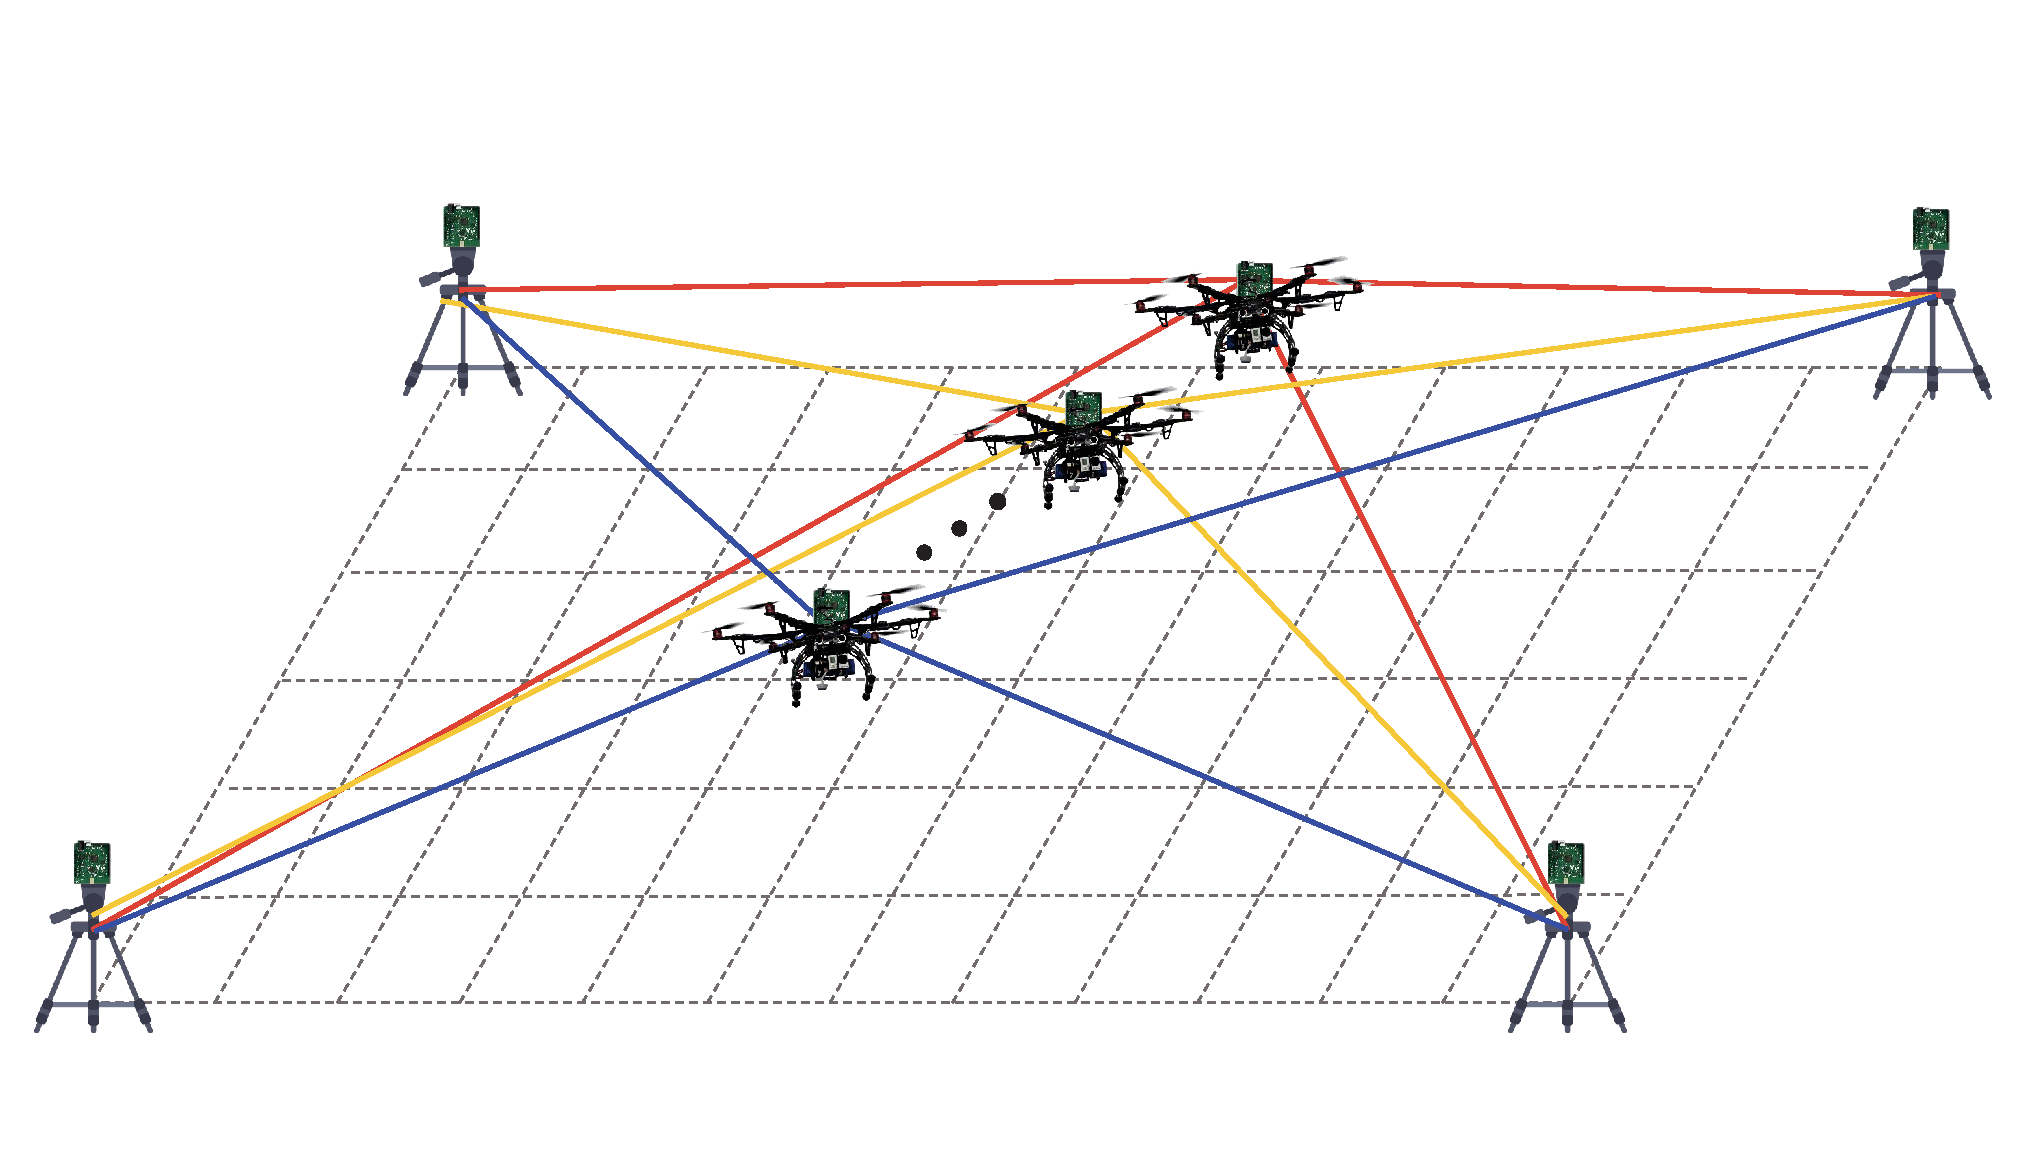
\includegraphics[height=4.5cm]{Drone_image_1}
	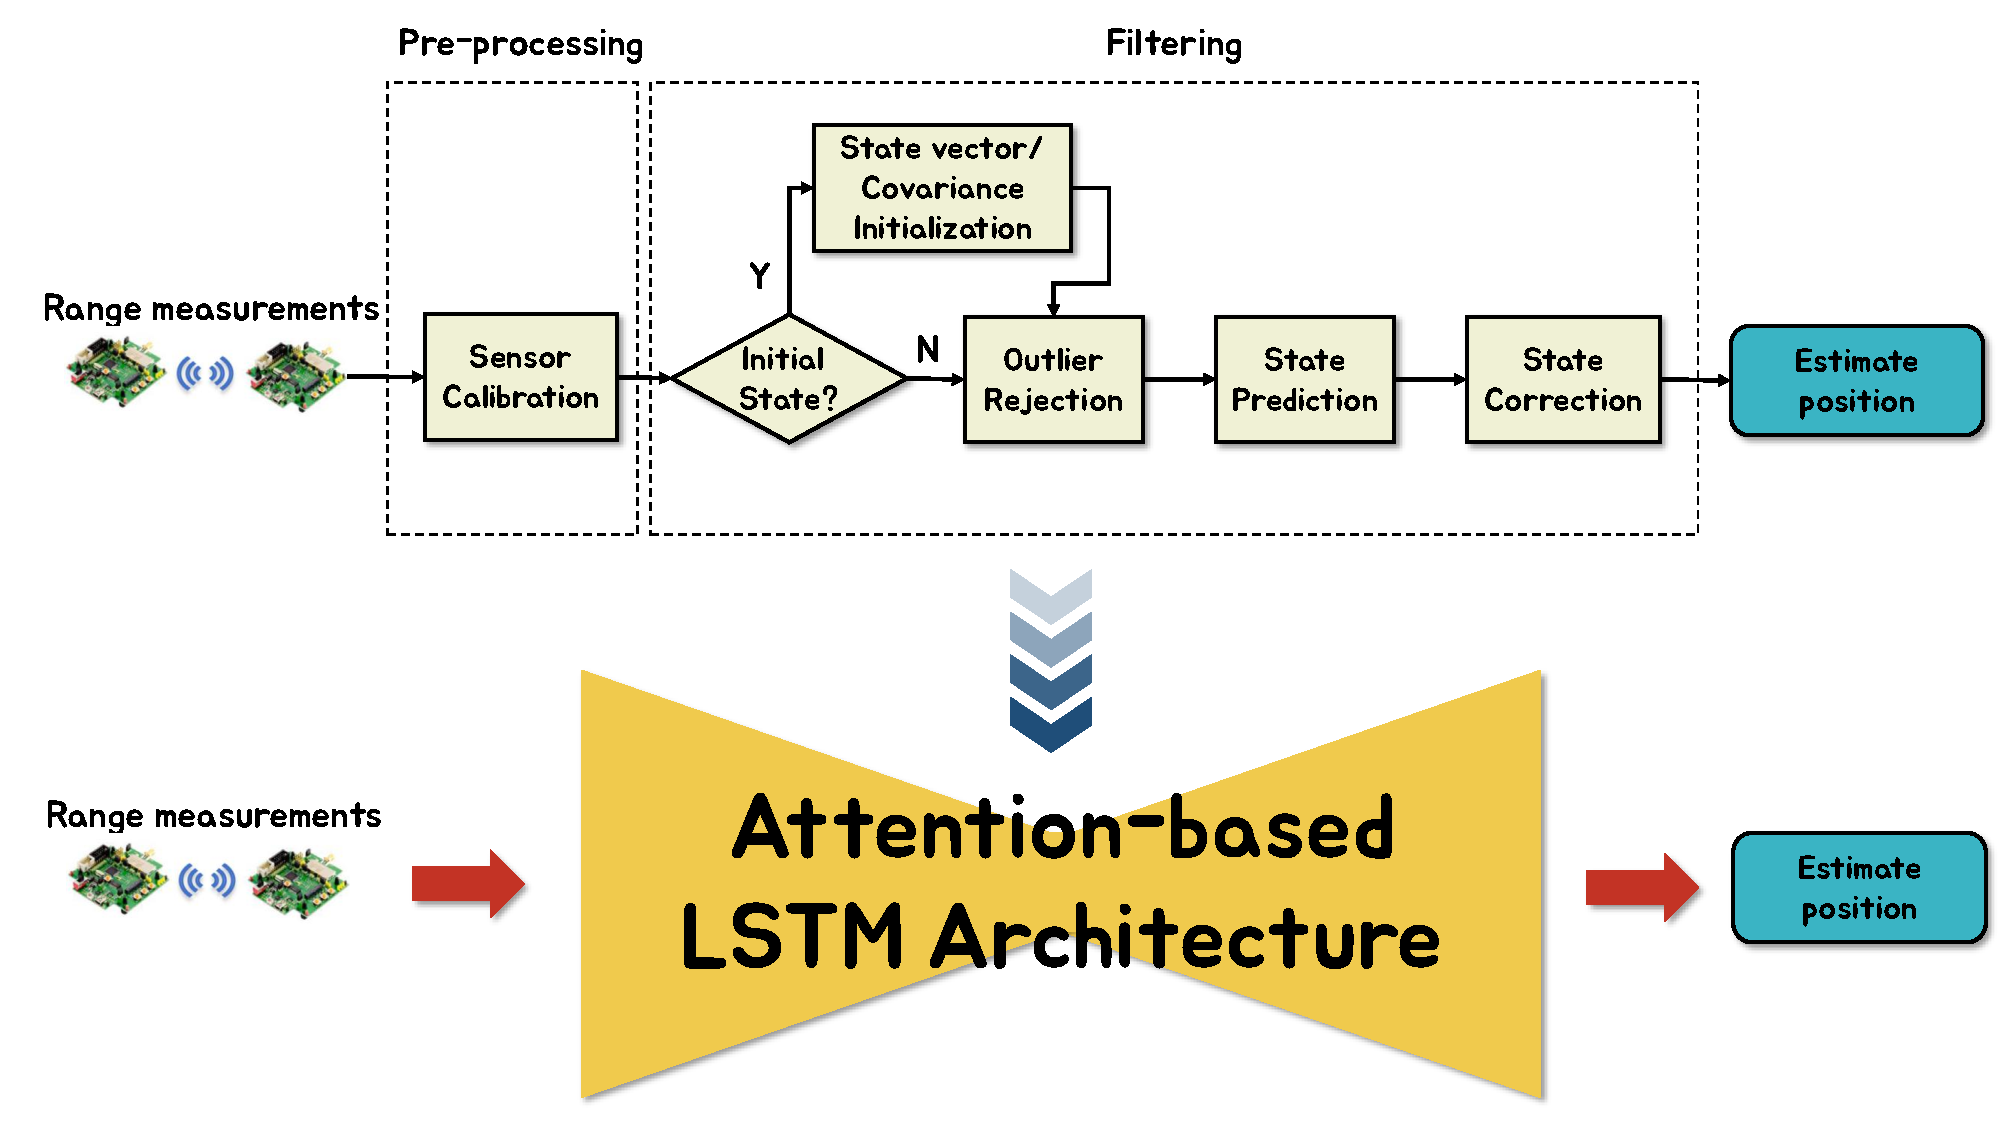
\includegraphics[height=5cm]{CE554_traditional_to_RNN}
	\label{fig:example}
	\caption{System overview. A robot localizes its own pose through distance data and the derivative of distance data. }
	
\end{figure}

\section{Related Works}

In this section, we briefly survey previous researches closely focused on 
Long Short-Term Memory(LSTM) model and applications of LSTMs to solve domain problems.

\subsubsection{LSTM}

LSTM is a type of Recurrent Neural Networks(RNNs) that has loops so that infer output based on not only the input data, but also the internal state formed by previous information. In other words, while the RNN deals with sequential data, the network has remembered the previous state generated by past inputs and might be able to output the present time step via internal state and input, which is very similar to filtering algorithms.

However, RNNs often have a \textit{vanishing gradient problem},i.e., RNNs fail to propagate the previous matter into present tasks as time step gap grows by. In other words, RNNs are not able to learn to store appropriate internal states and operate on long-term trends. That is the reason why the Long Short-Term Memory (LSTM) architecture was introduced to solve this long-term dependency problem and make the networks possible to learn longer-term contextual understandings\cite{hochreiter1997long}.
By virtue of the LSTM architecture that has memory gates and units that enable learning of long-term dependencies\cite{zaremba2014learning}, LSTM are widely used in most of the deep learning research areas and numerous variations of LSTM architecutres have been studied.

\begin{figure*}[ht]
	
	\centering
	%\subfigure[]{
	%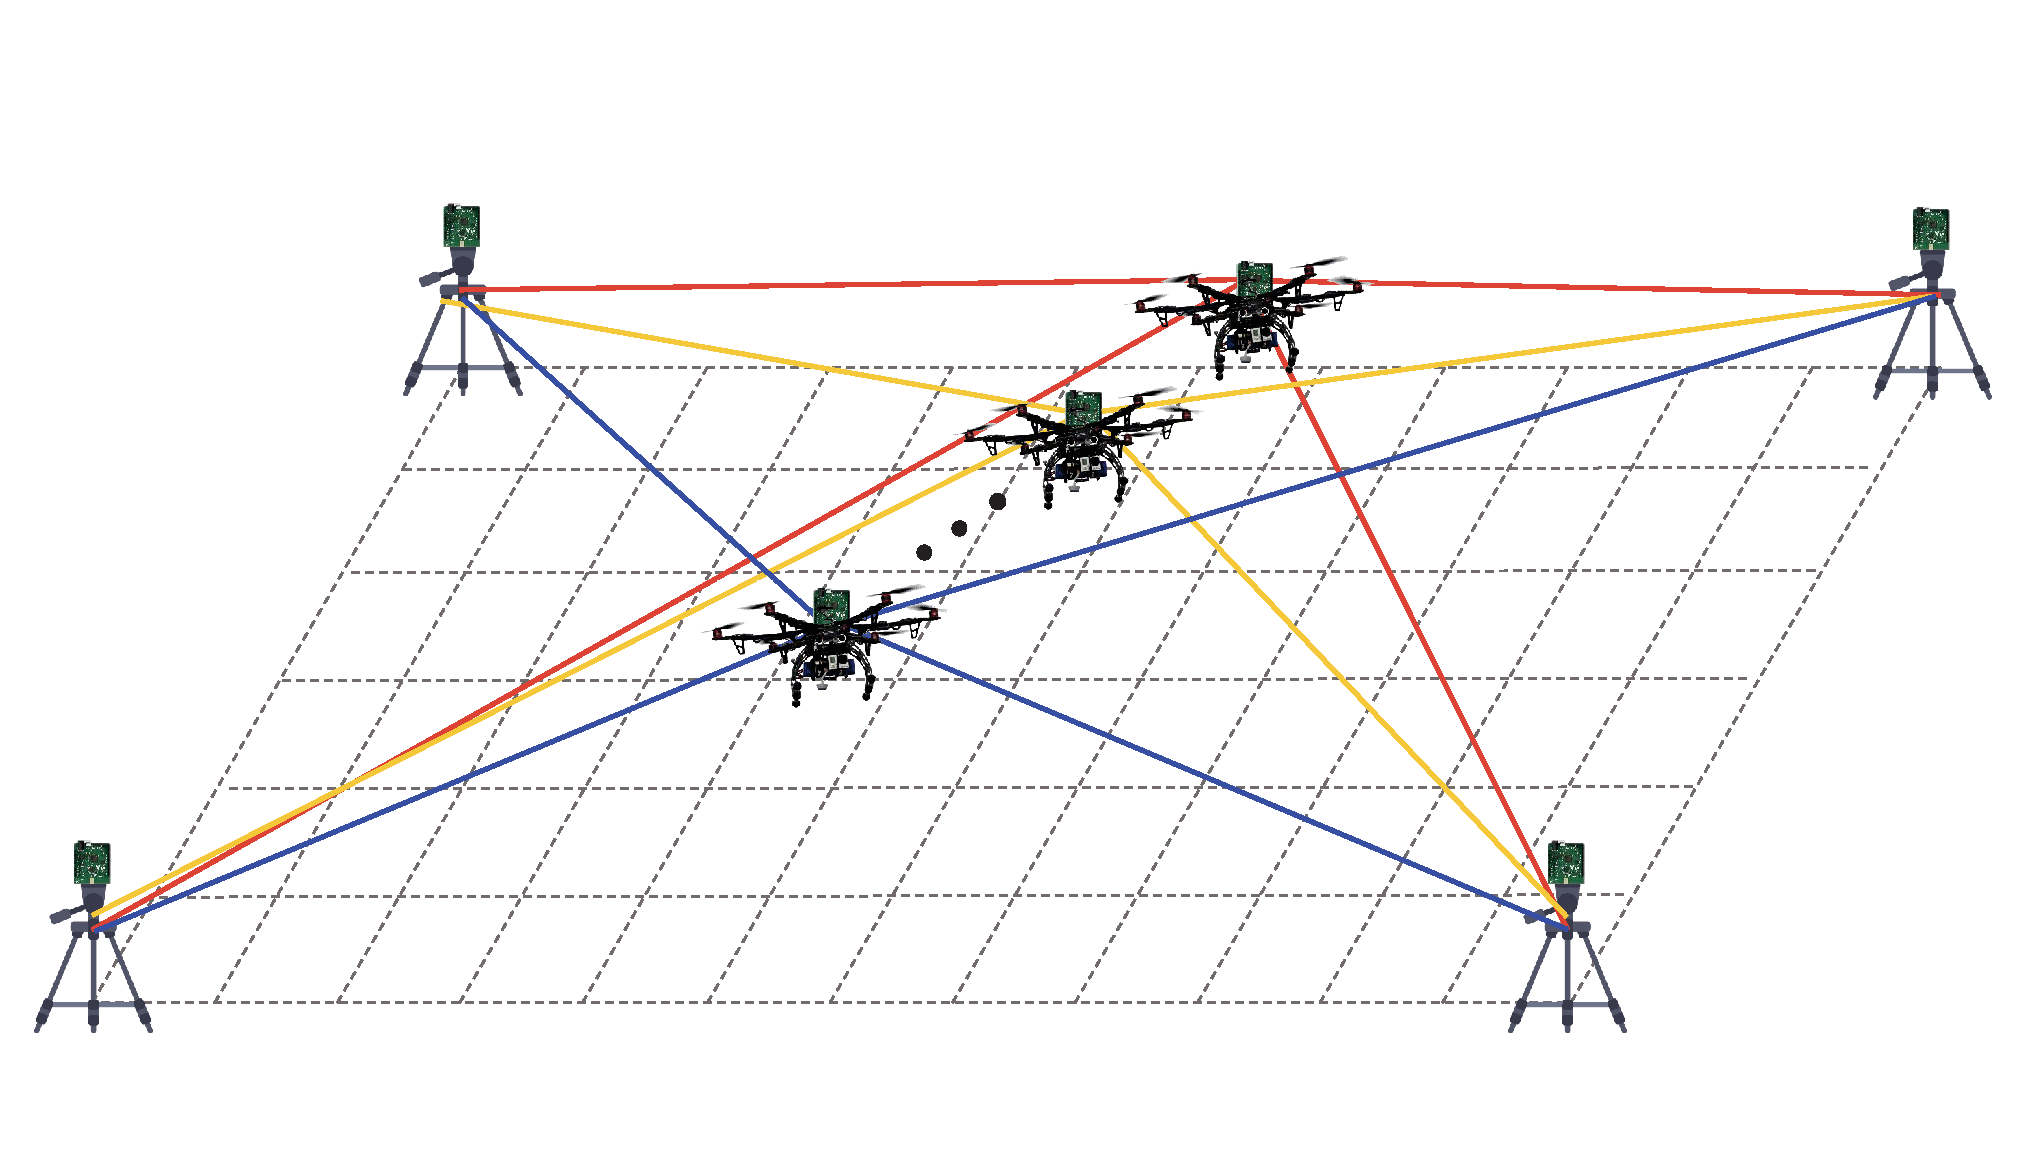
\includegraphics[height=4.5cm]{Drone_image_1}
	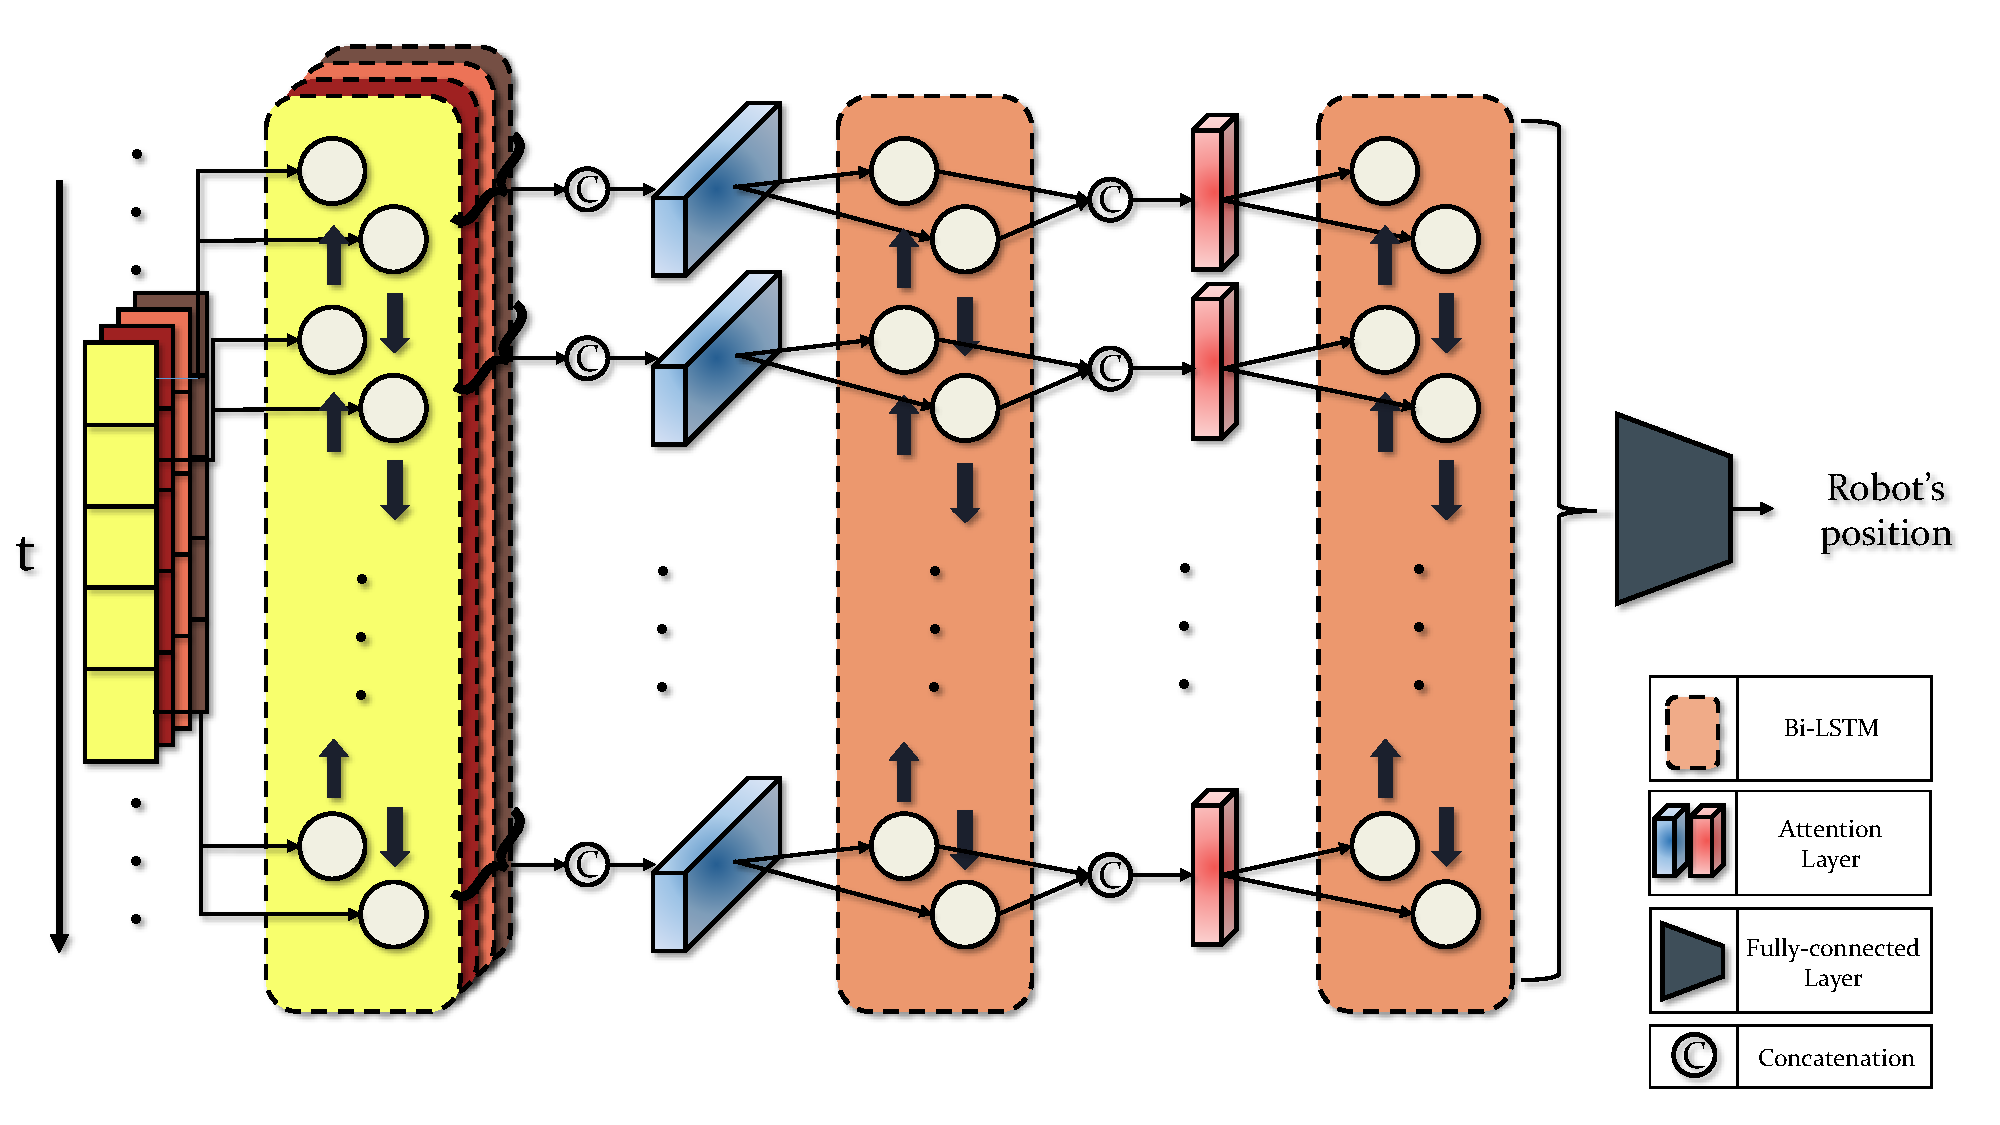
\includegraphics[height=10 cm]{CE554_networks}
	
	%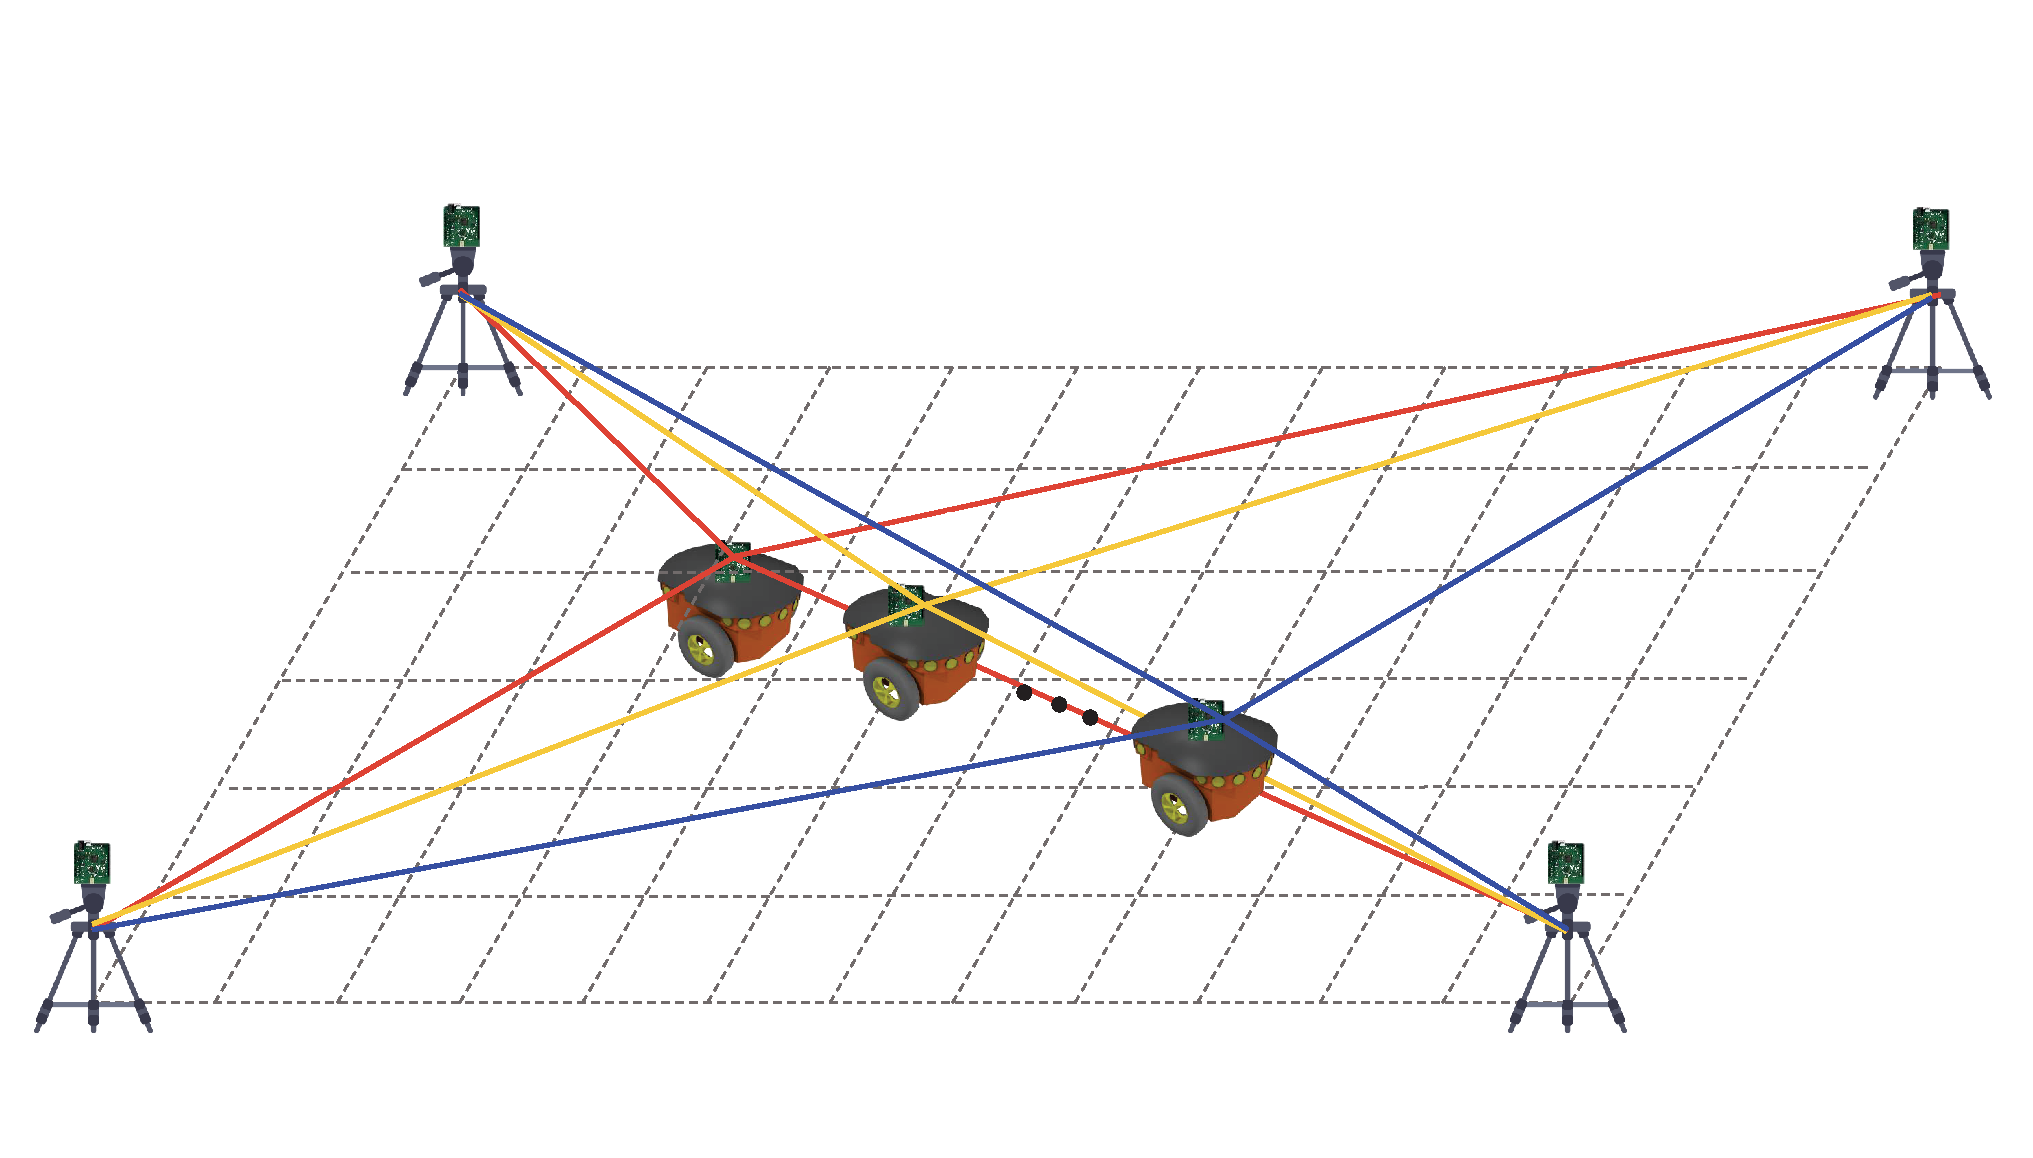
\includegraphics[trim={0 0 0 1cm}height=4.5cm]{IROS2018_image_1}
	\label{fig:example}
	%	}
	
	\caption{Blabla. }
	
\end{figure*}


\subsubsection{Localization with Deep Learning}
There have been many approaches combining Simultaneous Localization and Mapping (SLAM) with deep learning, aiming to overcome the limitations on SLAM only technique such as difficulty on tuning the proper parameters in different environments and recovering an exact scale. Actually, those researches are showing the superior performance to the traditional SLAM approaches.


One of the popular SLAM techniques with deep learning is CNN-SLAM \cite{tateno2017cnn} which takes Convolutional Neural Networks (CNNs) to precisely predict the depth from a single image without any scene-based assumptions or geometric constraints, allowing them to recover the absolute scale of the reconstruction. Another approach using deep learning for localization is Deep VO \cite{clark2017vinet} In this method, Recurrent Convolutional Neural Networks (RCNNs) is utilized. Specifically, feature representation is learned by Convolutional Neural Networks and Sequential information and motion dynamics are obtained by deep Recurrent Neural Networks without using any module in the classic VO pipeline.



\subsubsection{Applications of LSTMs}

There are many variations of LSTM architecture. As studies of deep learning are getting popular, various modified architectures of LSTM have been proposed for many tasks in a wide area of science and engineering. Because LSTM is powerful when dealing with sequential data and infering output by using previous inputs, LSTM is utilized to estimate pose by being attached to the end part of deep learning architecture \cite{wang2017deepvo, kendall2015posenet, turan2018deep}  as a stacked form of LSTM. In addition, LSTM takes many various data as input; LSTM is exploited for sequential modeling using LiDAR scan data \cite{gladh2016deep}, images \cite{walch2017image, wang2017deepvo}, IMU \cite{ordonez2016deep}, a fusion of IMU and images \cite{clark2017vinet}.


\section{Our approaches}
\subsection{LSTM}

\subsection{Bidirecional LSTM}

\subsection{Stacked Architecture}

\subsection{Multimodal Architecture}

\subsection{Training Loss}

We set the experiment on the virtual situation and generate distance data set which corresponds to the position with 10\% noise error and let RNN be trained using these distance data. Train data are just zigzag paths and test data is an arbitrary path, so we also check if RNN can estimate the position despite the variation of distance data as input.

Let $\Theta$ be the parameters of our RNN model, then our final goal is to find optimal parameters $\Theta^{*}$ for localization by minimizing Mean Square Error (MSE) of Euclidean distance between ground truth position $Y_k$ and estimated position $\hat{Y_k}$.

\begin{equation}
\Theta^{*} = \underset{\Theta}{\mathrm{argmin}} \sum_{k=1}^N \parallel Y_k - \hat{Y_k} \parallel^{2}
\end{equation}  


\section{Experiment}


\subsection{Experiment settings} 

Our experimental system consists of a UWB(ultra wideband) sensor tag and eight UWB sensor anchors that have a UWB transceiver, the motion capture system with 12 cameras, and a mobile robot and a small form-factor computer. The UWB tag and anchors are attached to a robot and landmarks respectively. The tag and anchor system operates like that an anchor transmits the Ultra wideband signal and a tag receives the signal and measures the range between two devices. Each UWB sensors have a UWB transceiver that is DW1000 UWB-chip made by Decawave and supports 6 RF bands from 3.5 GHz to 6.5 GHz and has centimeter-level accuracy. And The motion capture system is Eagle Digital Realtime system of motion analysis corporation that operates with the principle of stereo pattern recognition that is a kind of photogrammetry based on the epipolar geometry and the triangulation methodology. the system has < 1mm accuracy and > 500 frames/s frame rate. And a mobile robot is iClebo Kobuki from yujinrobot that has 70 cm/s maximum velocity. And the small form-factor computer is a gigabyte Ultra compact PC kit that CPU is intel dual core i7 / 2.7GHz and ram is DDR4SDRAM.
Deep learning framework used for our network is pytorch 0.4.0 on python 3.6. The network is trained on the machine that OS is Ubuntu mate 16.04 LTS and GPUs are gtx 1080ti and gtx titan. The network inferences on the same machine that we used for training.

\subsection{Training/Test Dataset}

Fig. \ref{setting} shows the description of experimental environment. The UWB tag and a small computer are attached to mobile robot. The UWB anchors are attached to stands that have two different heights and positioned randomly. Inside of the square space, a mobile robot goes on various random paths. And the distance data is measured by the UWB tag and the global position data is measured by the motion capture system. In the computer two different thread receive these two kinds of data separately. So, to synchronize these data, we make an independent thread that concatenates and saves these data and the thread is running at 20Hz frequency shown in Fig. 3. After the experiment, we separate the entire data to two types of dataset, some are the training datasets and others are test datasets. Each type of datasets is independent of each other.
\begin{figure}[h]
	\centering
	\begin{subfigure}[b]{.25\textwidth}
		\centering
		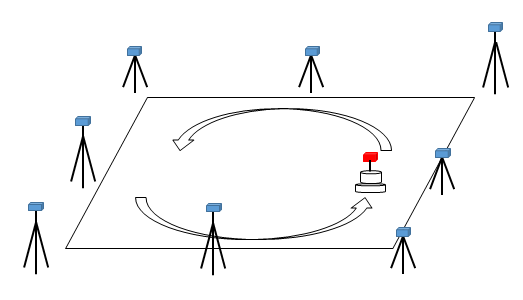
\includegraphics[width=.9\textwidth]{descriptionSystem}
		\label{setting:sub1} 	
		\caption{Description.}
	\end{subfigure}%
	\begin{subfigure}[b]{.25\textwidth}
		\centering
		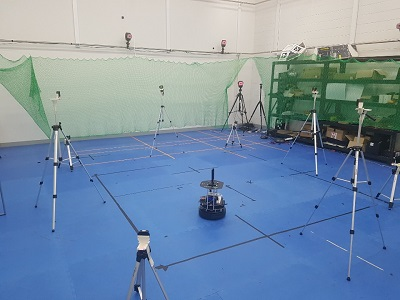
\includegraphics[width=.9\textwidth]{actualSystem}
		\label{setting:sub2} 	
		\caption{Actual.}
	\end{subfigure}
	\caption{Experimental system overview.}
	\label{setting}
	
\end{figure}
\begin{figure}[h]
	\centering
	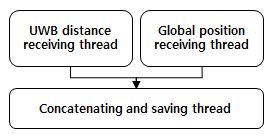
\includegraphics[width=.9\linewidth]{savingThread}
	\caption{Data syncronizing method.}
	\label{fig:sync}
\end{figure}

In addition, to use the distance data for traditional RO-slam we calibrate the distance from each anchors. As you can see in Fig. 4, we measure the data from a tag to each anchors at the points where the actual distance was measured by 1m, 2m, 3m, 4m. By using the linear regression, we compute the ratio between the measurement and the actual distance. And the ratios of each anchor are used to calibrate it.
\begin{figure}[h]
	\centering
	\begin{subfigure}[b]{.35\textwidth}
		\centering
		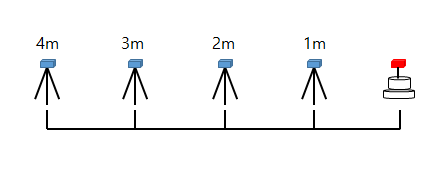
\includegraphics[width=.9\textwidth]{calib}
		\label{calibration:sub1} 	
		\caption{Description.}
	\end{subfigure}%
	\begin{subfigure}[b]{.15\textwidth}
		\centering
		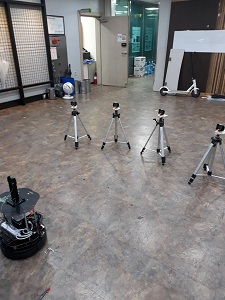
\includegraphics[width=0.9\textwidth]{calib2}
		\label{calibration:sub2} 	
		\caption{Actual}
	\end{subfigure}
	\caption{Sensor calibration overview.}
	\label{fig:test}
\end{figure} 

\section{Results}

To verify our proposal that RNNs can estimate the robot's position through varying range data, we trained our RNN-based multimodal architecture. Plus, to compare to previous traditional SLAM algorithm, we also estimate robot's position by particle filter(PF) based algorithm. Train data are our own data gathered by UWB sensors and motion capture camera, so neural networks take range-only measurements as input and outputs robot's position. Ground truth data is robot's position measured by eagle eye motion capturer, whose error is in mm units. The results of trajectory prediction are shown in Fig. \ref{fig:trajectory} and Root-Mean-Squared Error (RMSE) are shown in Table \ref{RMSE_table}.

\subsection{Analysis of errors}

 We set two test trajectory cases. However, unexpectedly, Performance of PF based localization is better than performance of our architecture. In case of GRU, it has only two gates which is less complex structure than LSTM \cite{chung2014empirical}. However, due to GRU's less complexity, GRU has less the number of neurons than LSTM so their non-linear mapping achieves less performance. Likewise, Bi-LSTM consists of two LSTMs to process sequence in two directions so that infer output using the correlation of the backward information and the forward information of the sequences of each time step with its two separate hidden layers. Thus, Bi-LSTM has better nonlinear mapping capability than LSTM. For similar reasons, stacked Bi-LSTM is the architecture that stacks two Bi-LSTMs, so inference performance is better than Bi-LSTM. As a result, the stacked Bi-LSTM showed the best performance among unit RNN architectures. Therefore, we can conclude that the performance improves as the non-linearity of the architecture increases.
 
 \begin{figure*}[h]
 	\centering
 	\begin{subfigure}[b]{.50\textwidth}
 		\centering
 		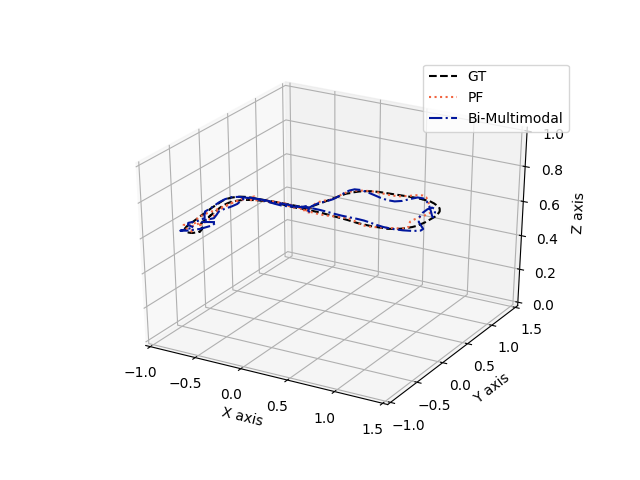
\includegraphics[width=.9\textwidth]{PF_multimodal_comparison1}
 		\label{fig:trajectory1} 	
 		\caption{Description.}
 	\end{subfigure}%
 	\begin{subfigure}[b]{.50\textwidth}
 		\centering
 		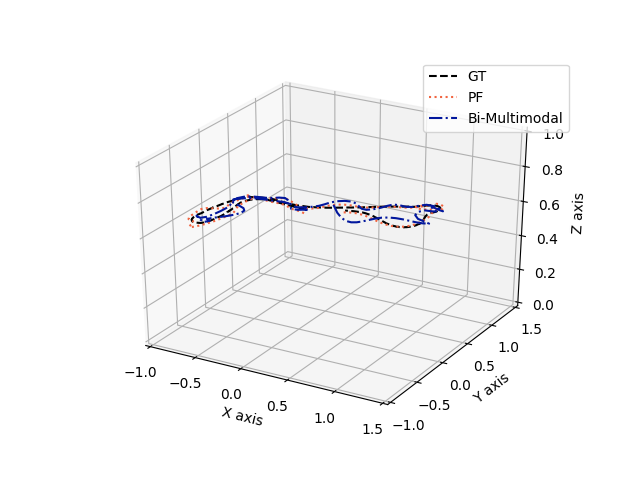
\includegraphics[width=0.9\textwidth]{PF_multimodal_comparison2}
 		\label{fig:trajectory2} 	
 		\caption{Actual}
 	\end{subfigure}
 	\caption{Sensor calibration overview.}
 	\label{fig:trajectory}
 \end{figure*} 
 
  \begin{figure*}[h]
 	\centering
 	\begin{subfigure}[b]{.50\textwidth}
 		\centering
 		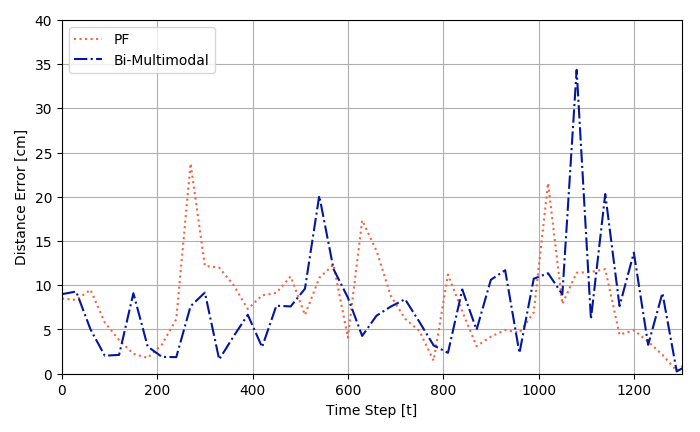
\includegraphics[width=.9\textwidth]{PF_multimodal_error1}
 		\label{fig:error1} 	
 		\caption{Description.}
 	\end{subfigure}%
 	\begin{subfigure}[b]{.50\textwidth}
 		\centering
 		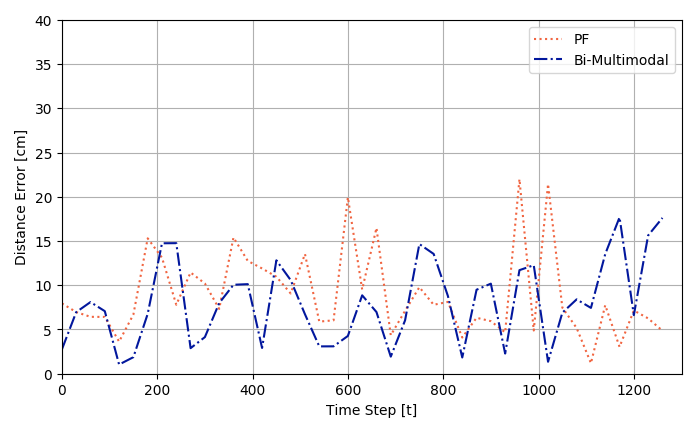
\includegraphics[width=0.9\textwidth]{PF_multimodal_error2}
 		\label{fig:error2} 	
 		\caption{Actual}
 	\end{subfigure}
 	\caption{Sensor calibration overview.}
 	\label{fig:error}
 \end{figure*} 
 
\begin{table}[h]
	\centering
	\begin{tabular}{cclcl}
		\hline
		\multicolumn{5}{c}{Results of RMSE{[}cm{]}}                                                                  \\ \hline
		\multicolumn{1}{c|}{Model}                    & \multicolumn{2}{c|}{Test1} & \multicolumn{2}{c}{Test2}      \\ \hline
		\multicolumn{1}{c|}{Particle filter-based}    & \multicolumn{2}{c|}{\textbf{9.1827}}     & \multicolumn{2}{c}{9.8803}          \\
		\multicolumn{1}{c|}{Bidirectional Multimodal} & \multicolumn{2}{c|}{11.3301}     & \multicolumn{2}{c}{\textbf{9.7528}}
	\end{tabular}
	\label{RMSE_table}
\end{table}


\section{Conclusion}

In this paper, we proposed a novel approach to range-only measurements localization using recurrent neural network models and tested various types of LSTM models for more accurate localization of the mobile robot. 

Using deep learning, our structure directly learns the end-to-end mapping between distance data and robot position. The stacked bidirectional LSTM structure exhibits the best estimates of robot positions than other RNN structure units. Therefore, we conclude that  the LSTM-based structure improves performance as non-linearity of structures increase and even if the robot position is not included in the ground truth dataset, our method is able to predict robot positions with small errors through sequential distance data. 

As a future work, because train/test dataset are generated on simulated environment, the proposed method needs to be tested in the real-world to check whether RNNs can deal with multipath problems and line of non-line of sight(NLOS) issues.
\bibliographystyle{IEEEtran}
% argument is your BibTeX string definitions and bibliography database(s)
\bibliography{./IEEEabrv,./MyBib}


\end{document}
